% Phasor Lock-in Derivation — temporal real-probe EP for the
%                              unit-circle (non-holomorphic) regime
% Compile standalone: pdflatex phasor_lockin_derivation.tex

\documentclass[11pt]{article}
\usepackage{amsmath,amssymb,amsthm}
\usepackage{bm}
\usepackage{booktabs}
\usepackage{enumitem}
\usepackage[margin=1in]{geometry}
\usepackage{hyperref}
\usepackage{tikz}
\usepackage{pgfplots}
\pgfplotsset{compat=1.16}
\usetikzlibrary{arrows.meta,decorations.pathmorphing,backgrounds,positioning,calc,patterns,fit}

% Shared figure palette
\definecolor{holo}{RGB}{30,110,190}     % holomorphic sideband / +omega_p
\definecolor{antiholo}{RGB}{200,80,30}  % anti-holomorphic sideband / -omega_p
\definecolor{probeC}{RGB}{40,140,90}    % probe waveform
\definecolor{basinC}{RGB}{90,150,200}   % good operating region
\definecolor{badC}{RGB}{200,120,120}    % failure regions
\definecolor{axisgray}{RGB}{110,110,110}

\newcommand{\R}{\mathbb{R}}
\newcommand{\C}{\mathbb{C}}
\newcommand{\T}{\mathbb{T}}
\newcommand{\im}{\mathrm{i}}
\newcommand{\dd}{\mathrm{d}}
\newcommand{\dt}{\Delta t}
\newcommand{\ie}{i.e.}
\newcommand{\eg}{e.g.}

\theoremstyle{definition}
\newtheorem{definition}{Definition}
\newtheorem{proposition}{Proposition}
\newtheorem{lemma}{Lemma}
\newtheorem{theorem}{Theorem}
\newtheorem{remark}{Remark}
\newtheorem{corollary}{Corollary}

\DeclareMathOperator{\diag}{diag}
\DeclareMathOperator{\Real}{Re}
\DeclareMathOperator{\Imag}{Im}

\title{Lock-in Equilibrium Propagation\\
for Phasor Networks (Temporal Real Probe)}
\author{}
\date{}

\begin{document}
\maketitle

\begin{abstract}
\noindent
Equilibrium propagation (EP) trains an energy-based network by
contrasting two settled states.  This note introduces \emph{lock-in
EP}, the variant needed when the neurons are \emph{phasors} ---
unit-modulus complex numbers living on a circle rather than real
activations on a line.  We assume the reader knows vanilla EP
(Scellier--Bengio) and focus on the single thing that genuinely
changes: the map from the nudge $\beta$ to the equilibrium state is no
longer holomorphic, so the standard two-phase (free/nudged) contrast
does not read off the gradient cleanly.  The remedy is to drive
$\beta$ as a small \emph{real cosine in time}, $\beta(t)=\varepsilon
\cos(\omega_p t)$, and recover the gradient by lock-in demodulation at
$+\omega_p$ in a single settle.  We build the method up from the
vanilla-EP picture, illustrate the settling dynamics, and defer the
heavier proofs to appendices.
\end{abstract}

\begin{center}\fbox{\parbox{0.95\linewidth}{\small
\textbf{Prerequisite:} vanilla equilibrium propagation. \quad
\textbf{Setting:} phasor networks on the unit circle
(non-holomorphic \emph{unit-projection} nonlinearity, real weights). \quad
\textbf{New ingredient:} a temporal real-probe lock-in,
$\beta(t)=\varepsilon\cos(\omega_p t)$, demodulated at $+\omega_p$,
replacing the two static free/nudged phases.\\[2pt]
\emph{Terminology.} Throughout, ``lock-in'' refers to the temporal
real-probe technique derived here.  The related \emph{spatial}
complex-$\beta$ method of holomorphic EP --- sampling $\beta$ on a
circle in the complex plane and taking a Fourier coefficient --- is
called the ``Cauchy contour,'' and is treated in the companion
holomorphic-EP derivation.
}}\end{center}

%======================================================================
\section{From Vanilla EP to Phasor EP}\label{sec:intro}
%======================================================================

Equilibrium propagation trains an energy-based network by letting it
settle to a \emph{free} equilibrium, nudging its output slightly toward
the target, letting it settle to a \emph{nudged} equilibrium, and
reading the parameter gradient off the difference between the two.
This note asks a single question: what changes when each neuron is a
\emph{phasor} --- a unit-modulus complex number $z=e^{\im\pi\theta}$
living on a circle --- instead of a real activation on a line?  The
answer is reassuring in shape and sharp in detail: the algorithm keeps
its two-phase form almost verbatim, but the mathematics of how the
gradient is extracted must change, because the phasor nonlinearity is
\emph{not holomorphic}.  Sections~\ref{sec:phasor-ep}%
--\ref{sec:grad} develop that change; this section sets up the picture.

\subsection{Vanilla EP in one page}\label{sec:vanilla}

Recall the standard construction.  A network has state $\bm{z}$,
parameters $\theta$, and a scalar energy $E(\bm{z},\theta)$ whose local
minima are the network's stable states.  Given an input, the
\emph{free} phase relaxes $\bm{z}$ to an equilibrium
$\bm{z}^*(0)=\arg\min_{\bm z} E$.  A cost $\mathcal{C}(\bm{z},\bm{y})$
measures output error, and the \emph{nudged} phase relaxes the
augmented energy $E + \beta\,\mathcal{C}$ to a second equilibrium
$\bm{z}^*(\beta)$ for a small real $\beta>0$.  The gradient theorem of
Scellier--Bengio then states
\begin{equation}\label{eq:vanilla-ep}
  \frac{\dd\mathcal{L}}{\dd\theta}
  \;=\;
  \lim_{\beta\to0}\frac{1}{\beta}
  \Bigl[
    \frac{\partial E}{\partial\theta}\Big|_{\bm{z}^*(\beta)}
    -
    \frac{\partial E}{\partial\theta}\Big|_{\bm{z}^*(0)}
  \Bigr],
\end{equation}
so a \emph{local, two-phase contrast} of a Hebbian quantity computes
the loss gradient --- no backward pass.  Everything below inherits this
skeleton; only the state space and the extraction of the limit
in~\eqref{eq:vanilla-ep} are new.

\subsection{What changes for phasors}\label{sec:whatchanges}

Three substitutions turn vanilla EP into phasor EP
(Figure~\ref{fig:statespace}):
\begin{enumerate}[label=(\roman*)]
\item \emph{State space.}  Real activations $\bm{z}\in\R^N$ become
  phasors on the torus $\T^N=\{z\in\C^N:|z_j|=1\}$.  The ``saturation''
  that a squashing nonlinearity provides in the real case is replaced
  by the \emph{topological} constraint $|z_j|=1$ --- a genuine
  nonlinearity with no saturating function and no bound to fight.
\item \emph{Coupling energy.}  Real quadratic couplings become the real
  part of a Hermitian form, $\Real\langle W\bm{z}_{\ell-1},\bm{z}_\ell
  \rangle$, which is exactly the channel-wise cosine similarity between
  the drive into a neuron and its state.
\item \emph{Cost.}  Mean-squared error becomes one-minus-similarity to
  a target phasor pattern, $\mathcal{C}=1-\tfrac1{d}\Real\langle
  \bm{z}_L,\bm{y}\rangle$, whose gradient is a constant pull toward
  $\bm{y}$ on the circle.
\end{enumerate}
The nonlinearity that enforces (i) is the entrywise \emph{unit
projector} $\mathrm{unit\_project}(z)=z/|z|$.  Because $|z|=\sqrt{z\bar
z}$ depends on $\bar z$, this map --- and hence the whole equilibrium
--- is not holomorphic in the state.  That single fact is the source of
everything distinctive about lock-in EP, and we return to it in
Section~\ref{sec:wirtinger}.

\begin{figure}[htbp]
\centering
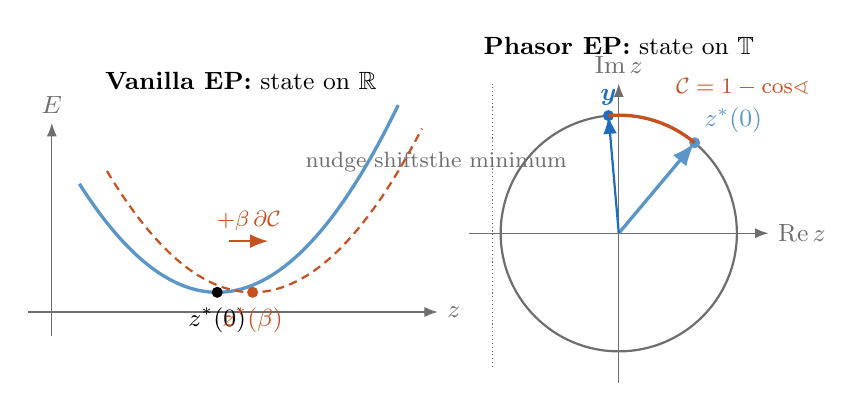
\begin{tikzpicture}[font=\small,>=Latex]
% ---------------- LEFT: vanilla EP on the line ----------------
\begin{scope}
  \node[anchor=south] at (2.4,2.7) {\textbf{Vanilla EP:} state on $\R$};
  \draw[->,axisgray] (-0.3,0)--(4.9,0) node[right]{$z$};
  \draw[->,axisgray] (0,-0.3)--(0,2.4) node[above]{$E$};
  % free energy bowl
  \draw[basinC,very thick,domain=0.35:4.4,samples=80,smooth]
     plot (\x,{0.45*(\x-2.1)^2+0.25});
  % free minimum
  \fill[black] (2.1,0.25) circle (2pt) node[below=2pt]{$z^*(0)$};
  % nudged bowl (shifted right toward target)
  \draw[antiholo,thick,densely dashed,domain=0.7:4.7,samples=80,smooth]
     plot (\x,{0.45*(\x-2.55)^2+0.25});
  \fill[antiholo] (2.55,0.25) circle (2pt) node[below=2pt]{$z^*(\beta)$};
  \draw[->,antiholo,thick] (2.25,0.9)--(2.75,0.9)
     node[midway,above]{\footnotesize $+\beta\,\partial\mathcal{C}$};
  \node[axisgray,anchor=west,font=\footnotesize] at (3.1,1.9)
     {nudge shifts\\ the minimum};
\end{scope}
\draw[axisgray,densely dotted] (5.6,-0.7)--(5.6,2.9);
% ---------------- RIGHT: phasor EP on the circle ----------------
\begin{scope}[xshift=7.2cm,yshift=1.0cm]
  \node[anchor=south] at (0,2.15) {\textbf{Phasor EP:} state on $\T$};
  \draw[axisgray,thick] (0,0) circle (1.5);
  \draw[->,axisgray] (-1.9,0)--(1.9,0) node[right]{$\Real z$};
  \draw[->,axisgray] (0,-1.9)--(0,1.9) node[above]{$\Imag z$};
  % free state
  \draw[->,basinC,very thick] (0,0)--(50:1.5);
  \fill[basinC] (50:1.5) circle (2pt) node[anchor=south west]{$z^*(0)$};
  % target
  \draw[->,holo,thick] (0,0)--(95:1.5);
  \fill[holo] (95:1.5) circle (2pt) node[anchor=south]{$\bm{y}$};
  % arc = cost
  \draw[antiholo,very thick] (50:1.5) arc (50:95:1.5);
  \node[antiholo,font=\footnotesize,anchor=west] at (72:1.95)
     {$\mathcal{C}=1-\cos\!\sphericalangle$};
\end{scope}
\end{tikzpicture}
\caption{The one conceptual substitution behind phasor EP.
\emph{Left:} vanilla EP lives on the real line; the free minimum
$z^*(0)$ of the energy bowl shifts to $z^*(\beta)$ when the output is
nudged toward the target, and~\eqref{eq:vanilla-ep} reads the gradient
off that shift.  \emph{Right:} a phasor neuron lives on the unit
circle; the state $z^*(0)$ is an \emph{angle}, the target $\bm{y}$ is
another angle, and the cost is the arc (cosine) distance between them.
The nudge rotates $z^*$ toward $\bm{y}$ along the circle instead of
sliding it along a line.}
\label{fig:statespace}
\end{figure}

\subsection{Settling dynamics}\label{sec:settling-intro}

In the free phase a phasor layer relaxes by a \emph{projected} flow:
starting from $\bm{z}=\bm{0}$, each step forms the complex drive from
the neighbouring layers, projects it back onto the unit circle, and
takes a small convex step toward it.  The state therefore travels
outward from the origin through the interior of the disk and curves
into a phase-consensus equilibrium on the circle
(Figure~\ref{fig:freesettle}); the interior iterates are transient and
only the equilibrium sits exactly on $\T$.  Viewed as a time series,
each channel's \emph{angle} converges to a plateau during the free
settle, and switching on the nudge shifts that plateau by a small
amount toward the target (Figure~\ref{fig:settle-ts}).  It is precisely
that small, $O(\beta)$ shift of the equilibrium that
both~\eqref{eq:vanilla-ep} and its lock-in replacement must measure
(Figure~\ref{fig:nudge-arc}).

\begin{figure}[htbp]
\centering
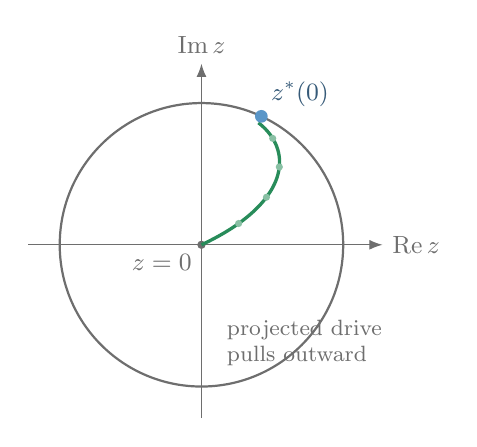
\begin{tikzpicture}[font=\small,>=Latex]
  \def\R{1.8}
  \draw[axisgray,thick] (0,0) circle (\R);
  \draw[->,axisgray] (-2.2,0)--(2.3,0) node[right]{$\Real z$};
  \draw[->,axisgray] (0,-2.2)--(0,2.3) node[above]{$\Imag z$};
  \fill[axisgray] (0,0) circle (1.5pt) node[anchor=north east]{$z=0$};
  % trajectory: radius grows 0 -> R while angle sweeps 25 -> 65 deg
  \draw[probeC,very thick,domain=0:1,samples=90,smooth,variable=\t]
     plot ({\R*(1-exp(-3.0*\t))*cos(25+40*\t)},
           {\R*(1-exp(-3.0*\t))*sin(25+40*\t)});
  % transient interior iterates
  \foreach \t in {0.12,0.28,0.5,0.78}{
    \fill[probeC!55] ({\R*(1-exp(-3.0*\t))*cos(25+40*\t)},
                      {\R*(1-exp(-3.0*\t))*sin(25+40*\t)}) circle (1.3pt);
  }
  \fill[basinC] (65:\R) circle (2.3pt);
  \node[basinC!60!black,anchor=south west] at (65:\R) {$z^*(0)$};
  \node[axisgray,anchor=west,font=\footnotesize,align=left] at (0.2,-1.25)
     {projected drive\\ pulls outward};
\end{tikzpicture}
\caption{Free-phase settling of a single hidden phasor.  The state
starts at the origin; each step projects the complex drive onto the
unit circle and steps toward it, so the trajectory (green) travels
\emph{outward} through the interior of the disk --- the transient
iterates (faint dots) lie strictly inside $|z|<1$ --- and curves onto
the free equilibrium $z^*(0)$, where the drift has become purely
radial.  Only the equilibrium sits exactly on the torus $\T$.}
\label{fig:freesettle}
\end{figure}

\begin{figure}[htbp]
\centering
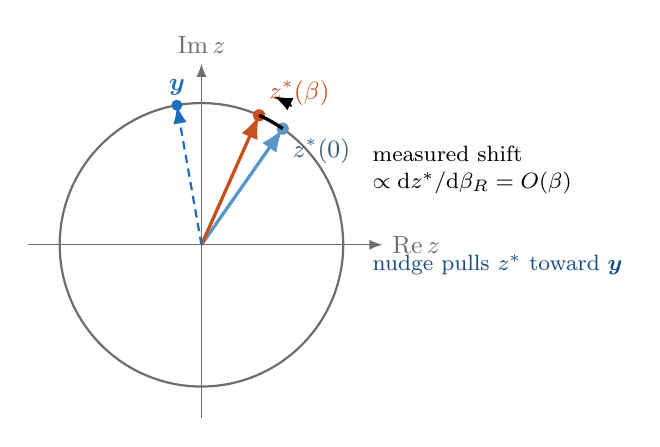
\begin{tikzpicture}[font=\small,>=Latex]
  \def\R{1.8}
  \draw[axisgray,thick] (0,0) circle (\R);
  \draw[->,axisgray] (-2.2,0)--(2.3,0) node[right]{$\Real z$};
  \draw[->,axisgray] (0,-2.2)--(0,2.3) node[above]{$\Imag z$};
  \draw[->,basinC,very thick] (0,0)--(55:\R);
  \fill[basinC] (55:\R) circle (2.2pt);
  \node[basinC!60!black,anchor=north west] at (55:\R) {$z^*(0)$};
  \draw[->,antiholo,very thick] (0,0)--(66:\R);
  \fill[antiholo] (66:\R) circle (2.2pt);
  \node[antiholo,anchor=south west] at (66:\R) {$z^*(\beta)$};
  \draw[->,holo,thick,densely dashed] (0,0)--(100:\R);
  \fill[holo] (100:\R) circle (2pt);
  \node[holo,anchor=south] at (100:\R) {$\bm{y}$};
  \draw[very thick] (55:\R) arc (55:66:\R);
  \draw[->,thick] (57:2.1) arc (57:64:2.1);
  \node[anchor=west,font=\footnotesize,align=left] at (2.05,0.95)
     {measured shift\\ $\propto \dd z^*/\dd\beta_R=O(\beta)$};
  \node[holo!70!black,font=\footnotesize,anchor=west] at (2.05,-0.25)
     {nudge pulls $z^*$ toward $\bm{y}$};
\end{tikzpicture}
\caption{What the two-phase contrast measures.  The nudge rotates the
free equilibrium $z^*(0)$ a small arc toward the target $\bm{y}$,
reaching $z^*(\beta)$.  Vanilla EP reads the gradient off this
$O(\beta)$ displacement via~\eqref{eq:vanilla-ep}; lock-in EP measures
the same displacement, but as the amplitude of a modulation rather than
a static difference (Section~\ref{sec:probe}).}
\label{fig:nudge-arc}
\end{figure}

\begin{figure}[htbp]
\centering
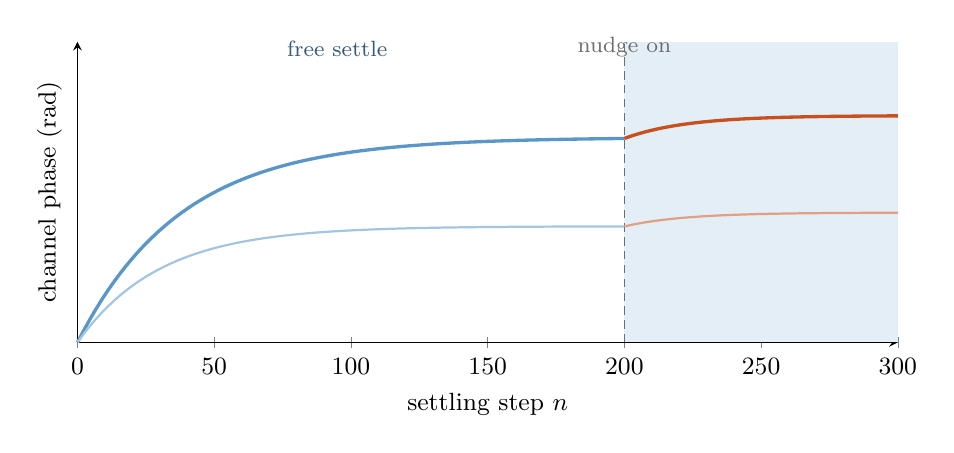
\begin{tikzpicture}[font=\small]
\begin{axis}[
   width=12cm,height=5.4cm,
   xlabel={settling step $n$},
   ylabel={channel phase (rad)},
   xmin=0,xmax=300,ymin=0,ymax=2.2,
   ytick=\empty,
   axis lines=left,
   clip=false,
]
  \fill[holo!12] (axis cs:200,0) rectangle (axis cs:300,2.2);
  \draw[axisgray,densely dashed] (axis cs:200,0)--(axis cs:200,2.2);
  \node[anchor=south,axisgray,font=\footnotesize] at (axis cs:200,2.02){nudge on};
  \node[anchor=south,basinC!60!black,font=\footnotesize] at (axis cs:95,2.02){free settle};
  \addplot[basinC,very thick,domain=0:200,samples=90]{1.5*(1-exp(-x/38))};
  \addplot[antiholo,very thick,domain=200:300,samples=60]
     {1.5*(1-exp(-x/38))+0.16*(1-exp(-(x-200)/22))};
  \addplot[basinC!55,thick,domain=0:200,samples=90]{0.85*(1-exp(-x/30))};
  \addplot[antiholo!55,thick,domain=200:300,samples=60]
     {0.85*(1-exp(-x/30))+0.10*(1-exp(-(x-200)/22))};
\end{axis}
\end{tikzpicture}
\caption{Settling as a time series.  During the free phase
($\beta=0$) each channel's phase relaxes to a plateau $z^*(0)$; when the
nudge switches on (shaded) the plateau shifts by a small $O(\beta)$
amount to $z^*(\beta)$.  Lock-in EP replaces the abrupt switch with a
gentle cosine modulation of $\beta$ and reads the gradient from the
amplitude of the resulting oscillation of these plateaus.}
\label{fig:settle-ts}
\end{figure}

\subsection{The one new complication, and the fix}\label{sec:complication}

Here is the wrinkle that the rest of the note resolves.  Because the
unit projector is not holomorphic, perturbing the equilibrium by a
nudge produces \emph{two} first-order responses, not one: a
``holomorphic'' part $\partial\bm{z}^*/\partial\beta$ and an
``anti-holomorphic'' part $\partial\bm{z}^*/\partial\bar\beta$
(Section~\ref{sec:wirtinger}).  The gradient on real weights needs
their \emph{sum}, the real-axis directional derivative
$\dd\bm{z}^*/\dd\beta_R$.  Driving the nudge as a real cosine in time,
$\beta(t)=\varepsilon\cos(\omega_p t)$, excites both responses
coherently at the probe frequency, and a single lock-in demodulation at
$+\omega_p$ returns exactly that sum
(Section~\ref{sec:probe}--\ref{sec:grad}).  The remainder of the note
makes this precise: Section~\ref{sec:phasor-ep} sets up the phasor
energy and its equilibria; Section~\ref{sec:wirtinger} pins down the
non-holomorphicity; Sections~\ref{sec:probe}--\ref{sec:demod} build the
probe and its demodulation; Section~\ref{sec:grad} states the gradient
formula; and Sections~\ref{sec:knobs}--\ref{sec:rel} cover tuning and
the relationship to other EP variants.  Heavier proofs are collected in
Appendices~\ref{app:stationarity}--\ref{app:sidebands}.

%======================================================================
\section{The Phasor Energy and Its Equilibria}\label{sec:phasor-ep}
%======================================================================

\subsection{State space and energy}

A phasor network of $L$ layers has hidden state
$\bm{z}_\ell \in \T^{d_\ell} \subset \C^{d_\ell}$ on the torus
$\T^{d_\ell} = \{z\in\C^{d_\ell} : |z_j|=1 \text{ for all } j\}$,
real weight matrices
$W_\ell \in \R^{d_\ell \times d_{\ell-1}}$, and per-channel
oscillator eigenvalues $\bm{k}_\ell = \bm{\lambda}_\ell + \im\bm{\omega}_\ell$
with $\lambda_{\ell,c} < 0$.  The input $\bm{x} = \bm{z}_0$ is fixed
and the dynamics are constrained to the torus by the entrywise
\emph{unit projector}
\begin{equation}\label{eq:unit-project}
  \mathrm{unit\_project}(z)
  \;=\; \frac{z}{|z|}
  \;=\; \frac{z}{\sqrt{z\bar z}},
  \qquad z \in \C.
\end{equation}

The Hopfield-style energy with self-energy and Hermitian inner
product $\langle\bm{u},\bm{v}\rangle = \sum_j \bar u_j\, v_j$ is
\begin{equation}\label{eq:energy}
  \Phi(\bm{z},\theta,\beta)
  \;=\;
  \sum_{\ell=1}^{L}
    \Bigl[
      \tfrac{1}{2}\,\Real\!\langle\bm{z}_\ell,\,K_\ell\bm{z}_\ell\rangle
      \;+\;
      \Real\!\langle W_\ell\bm{z}_{\ell-1},\,\bm{z}_\ell\rangle
    \Bigr]
  \;-\;
  \beta\,\mathcal{C}(\bm{z}_L,\,\bm{y}),
\end{equation}
where $K_\ell = \diag(\bm{k}_\ell)$, $\theta=\{W_\ell\}$ collects the
trainable parameters, and $\mathcal{C}$ is the task cost.

\begin{remark}[Two inner-product conventions]
The Hermitian inner product in~\eqref{eq:energy} is the natural choice
for a network whose states live on the unit circle: $\Real\langle u,v\rangle
= \tfrac{1}{2}(u^H v + v^H u)$ is the real, unit-circle cosine
similarity that the codebook similarity cost
$\mathcal{C}(\bm{z}_L,\bm{y}) = 1 - \tfrac{1}{d_L}\Real\langle\bm{z}_L,\bm{y}\rangle$
also uses.  This differs from the bilinear form
$\langle u,v\rangle_\mathrm{bi}=\sum_j u_j v_j$ used in the
holomorphic-regime (companion) derivation;
the Hermitian convention is what allows the unit-circle constraint to
sit comfortably inside the energy at the cost of breaking
holomorphicity in $\bm{z}$.
\end{remark}

\subsection{The settling drift and its equilibria}

The settling is a \emph{projected quasi-gradient flow} on $\Phi$: in
the default configuration the drift is exactly (twice) the Wirtinger
gradient of $\Phi$, and the variant that folds in the oscillator
self-force additionally contains a non-variational rotational component
(Appendix~\ref{app:stationarity}).  The drift is
\begin{equation}\label{eq:settle-grad}
  \bm{g}_\ell
  \;=\;
  \tfrac{1}{2}K_\ell\bm{z}_\ell
  \;+\;
  W_\ell\bm{z}_{\ell-1}
  \;+\;
  W_{\ell+1}^{\!\top}\bm{z}_{\ell+1}
  \;-\;
  2\beta\,\delta_{\ell L}\,
  \frac{\partial\mathcal{C}}{\partial\bar{\bm{z}}_L},
\end{equation}
where the self-force $\tfrac12 K_\ell\bm{z}_\ell$ is present only in the
variant that folds the oscillator dynamics into the drift; the default
and benchmarked configuration drops it, so the $K$ term is absent
entirely.  The cost term uses the \emph{real-parameter convention}
$\mathrm{nudge} = (\beta/d_L)\,\bm{y}
= -2\beta\,\partial\mathcal{C}/\partial\bar{\bm{z}}_L$ for the
similarity cost, deliberately carrying no factor of $\tfrac12$; this is
the convention that makes the estimator match finite differences on
real weights without a stray factor of two
(Appendix~\ref{app:stationarity}).
Discrete settling step (the projection is applied to the \emph{drive},
then convex-combined with the state):
\begin{equation}\label{eq:settle-step}
  \bm{z}_\ell^{(n+1)}
  \;=\;
  (1-\dt)\,\bm{z}_\ell^{(n)}
  \;+\;
  \dt\;\mathrm{unit\_project}\!\bigl(\bm{g}_\ell^{(n)}\bigr),
  \qquad
  \bm{g}_\ell^{(n)} = \bm{g}_\ell\bigr|_{\bm{z}^{(n)}}.
\end{equation}
Interim iterates therefore lie in the closed unit polydisk rather
than on the torus itself (states are initialized at $\bm{0}$ and the
projected drive pulls them outward); only equilibria sit exactly on
$\T^{d_\ell}$.  A fixed point of~\eqref{eq:settle-step} satisfies
$\bm{z}_\ell^* = \mathrm{unit\_project}(\bm{g}_\ell^*)$, hence
\begin{equation}\label{eq:radial-fp}
  \bm{g}_\ell^* \;=\; \bm{\mu}_\ell\odot\bm{z}_\ell^*,
  \qquad \bm{\mu}_\ell = |\bm{g}_\ell^*| \in \R_{\ge 0}^{d_\ell}
  \quad\text{(independent of $\dt$)}:
\end{equation}
\emph{the drift at equilibrium is purely radial.}  This defines the
free equilibrium $\bm{z}^*(0)$ at $\beta=0$ and the $\beta$-dependent
family $\bm{z}^*(\beta)$ when $\beta \ne 0$.

The implemented drift~\eqref{eq:settle-grad} is not quite the Wirtinger
gradient of the energy~\eqref{eq:energy}.  In the benchmarked
configuration it equals that gradient exactly up to an overall factor
of two,~\eqref{eq:drift-is-2grad}, which rescales the flow without
moving its fixed points; the variant that folds in the oscillator
self-force instead adds a non-variational \emph{rotational} term that
is tangential to the torus.
Appendix~\ref{app:stationarity} carries out the full decomposition:
the term-wise bookkeeping (including why the real-parameter nudge
convention avoids a stray factor of two) and the rotational component
together with its rotating-frame reduction for uniform $\bm{\omega}$.

\begin{lemma}[Stationarity at the projected equilibrium]
\label{lem:stationarity}
Suppose the drift is variational up to a radial term,
$\bm{g}_\ell = c\,\partial\Phi/\partial\bar{\bm{z}}_\ell
+ \bm{r}_\ell$ with $c>0$ and
$\bm{r}_\ell = \bm{\mu}'_\ell\odot\bm{z}_\ell$, $\bm{\mu}'_\ell$ real
(in the benchmarked configuration this holds exactly with $c=2$ and
$\bm{r}_\ell=\bm{0}$ by~\eqref{eq:drift-is-2grad}; the self-force
variant requires the $\bm{\omega}=\bm{0}$ or rotating-frame reduction
of Appendix~\ref{app:stationarity}).  Then at a projected fixed point,
\[
  \frac{\partial\Phi}{\partial\bar{\bm{z}}_\ell}\bigg|_{\bm{z}^*}
  \;=\; \bm{\nu}_\ell\odot\bm{z}^*_\ell,
  \qquad \bm{\nu}_\ell\in\R^{d_\ell}
  \quad\text{(the residual gradient is radial)},
\]
and consequently, since every smooth variation that stays on the torus
is tangential ($\Real(\bar z^*_j\,\delta z_j)=0$; in particular
$\delta\bm{z} = (\dd\bm{z}^*/\dd\theta)\,\delta\theta$ and
$\delta\bm{z} = (\dd\bm{z}^*/\dd\beta_R)\,\delta\beta_R$),
\begin{equation}\label{eq:envelope}
  \frac{\dd}{\dd\theta}\,\Phi\bigl(\bm{z}^*(\theta,\beta),\theta,\beta\bigr)
  \;=\;
  \frac{\partial\Phi}{\partial\theta}\bigg|_{\bm{z}^*},
  \qquad
  \frac{\dd}{\dd\beta_R}\,\Phi\bigl(\bm{z}^*,\theta,\beta\bigr)
  \;=\;
  -\,\mathcal{C}\bigl(\bm{z}^*_L,\bm{y}\bigr).
\end{equation}
\end{lemma}
\noindent\emph{Proof.} See Appendix~\ref{app:stationarity}.

\subsection{Standard (static) EP}

For real $\beta$ the Scellier--Bengio gradient theorem gives
\begin{equation}\label{eq:static-ep}
  \frac{\dd\mathcal{L}}{\dd\theta}
  \;=\;
  \lim_{\beta \to 0}\;\frac{1}{\beta}\!\left[
    \left.\frac{\partial\Phi}{\partial\theta}\right|_{\bm{z}^*(\beta)}
    -
    \left.\frac{\partial\Phi}{\partial\theta}\right|_{\bm{z}^*(0)}
  \right],
\end{equation}
with the corresponding two-phase Hebbian estimator
$\Delta W_\ell \propto -\bigl(\mathrm{hebb}_\ell^{\text{nudge}} - \mathrm{hebb}_\ell^{\text{free}}\bigr)/\beta$
(the two-phase static estimator).  On the constrained state space,
\eqref{eq:static-ep} rests on the envelope
property~\eqref{eq:envelope}: the Scellier--Bengio argument
differentiates $\Phi$ at a \emph{stationary} point, whereas the
projected equilibrium is stationary only up to a radial residual —
Lemma~\ref{lem:stationarity} shows this residual is invisible to
tangential variations, so the theorem carries over (under the
variational-drift reduction of Appendix~\ref{app:stationarity}).
Finite $\beta$ introduces
$O(\beta)$ bias from the nonlinearity of $\bm{z}^*(\beta)$; the
small-$\beta$ / large-bias trade-off is what holomorphic EP and lock-in
EP (this note) each address differently.

%======================================================================
\section{Wirtinger Calculus and Non-Holomorphicity}\label{sec:wirtinger}
%======================================================================

\subsection{Wirtinger derivatives}

For a smooth function $f(\beta,\bar\beta)$ of a complex variable
$\beta = \beta_R + \im\beta_I$ (treating $\beta$ and $\bar\beta$ as
independent),
\begin{equation}\label{eq:wirtinger}
  \frac{\partial}{\partial\beta}
  \;=\; \tfrac{1}{2}\!\left(\frac{\partial}{\partial\beta_R}
                          - \im\frac{\partial}{\partial\beta_I}\right),
  \qquad
  \frac{\partial}{\partial\bar\beta}
  \;=\; \tfrac{1}{2}\!\left(\frac{\partial}{\partial\beta_R}
                          + \im\frac{\partial}{\partial\beta_I}\right).
\end{equation}
The function is \emph{holomorphic} iff $\partial f/\partial\bar\beta = 0$
(the Cauchy--Riemann condition).  The real-axis directional derivative
is
\begin{equation}\label{eq:real-dir}
  \frac{\dd}{\dd\beta_R} f
  \;=\;
  \frac{\partial f}{\partial\beta} + \frac{\partial f}{\partial\bar\beta},
\end{equation}
and the imaginary-axis directional derivative is
\begin{equation}\label{eq:imag-dir}
  \frac{\dd}{\dd\beta_I} f
  \;=\;
  \im\!\left(\frac{\partial f}{\partial\beta} - \frac{\partial f}{\partial\bar\beta}\right).
\end{equation}

\subsection{Non-holomorphicity of unit projection}

\begin{proposition}\label{prop:nonholo}
The unit projector~\eqref{eq:unit-project} is not holomorphic in
$z$:
\[
  \frac{\partial}{\partial \bar z}\!\left(\frac{z}{|z|}\right)
  \;=\; -\frac{z}{2|z|^3} \cdot z
  \;=\; -\frac{z^2}{2|z|^3} \ne 0.
\]
\end{proposition}
\begin{proof}
Write $z/|z| = z\,(z\bar z)^{-1/2}$.  In the Wirtinger sense $z$ is
independent of $\bar z$, so
\[
  \frac{\partial}{\partial\bar z}\Bigl(z\,(z\bar z)^{-1/2}\Bigr)
  \;=\;
  z\cdot\Bigl(-\tfrac12\Bigr)(z\bar z)^{-3/2}\cdot z
  \;=\;
  -\frac{z^2}{2|z|^3}.
  \qedhere
\]
\end{proof}

\begin{corollary}\label{cor:nonholo-z*}
The equilibrium map $\bm{z}^*$ of~\eqref{eq:settle-step} is a smooth
function of $(\beta, \bar\beta)$ jointly, not a holomorphic function
of $\beta$.  In particular,
$\partial \bm{z}^* / \partial \bar\beta \ne 0$ in general, so the
chain rule for any observable $f(\bm{z}^*(\beta,\bar\beta))$ at
$\beta = 0$ reads
\begin{equation}\label{eq:dz-wirtinger}
  \bm{z}^*(\beta) - \bm{z}^*(0)
  \;=\;
  \beta\,
  \frac{\partial\bm{z}^*}{\partial\beta}\bigg|_0
  \;+\;
  \bar\beta\,
  \frac{\partial\bm{z}^*}{\partial\bar\beta}\bigg|_0
  \;+\;
  O(|\beta|^2),
\end{equation}
with both Wirtinger sidebands present.
\end{corollary}

\subsection{Why the spatial Cauchy contour misses the target}

The spatial Cauchy contour estimator of holomorphic EP evaluates
$\partial\Phi/\partial\theta$ at $\beta_n = r\,e^{2\pi\im n/N}$ and
takes the first Fourier coefficient $(1/N)\sum_n
\partial\Phi/\partial\theta|_{\bm{z}^*(\beta_n)}\cdot e^{-2\pi\im n/N}$.

The obstruction is subtler than a contamination.  The
anti-holomorphic sideband is in fact annihilated \emph{exactly} at
first order by the discrete Fourier sum for every $N\ge3$, so the
contour does not fail by leakage.  It fails by converging cleanly to
the \emph{wrong target} --- the holomorphic Wirtinger derivative
$\partial\bm{z}^*/\partial\beta$ rather than the real-axis directional
derivative $\dd/\dd\beta_R=\partial_\beta+\partial_{\bar\beta}$
\eqref{eq:real-dir} that EP on real parameters needs --- and by
retaining an aliased $O(r^2)$ mixed-term bias of the same order as the
temporal probe's own curvature bias.  It \emph{can} be repaired, by
demodulating the same samples against both $e^{\mp\im\varphi_n}$ and
adding, at the cost of a second accumulator and a coherent combination
(Appendix~\ref{app:sidebands}; Proposition~\ref{prop:cplx-fail} gives
the temporal analogue).  The temporal real probe's advantage is
therefore operational --- a single real drive and a single accumulator
deliver $\dd/\dd\beta_R$ directly, with the narrowband noise rejection
of lock-in detection --- rather than a matter of possibility.

\begin{figure}[htbp]
\centering
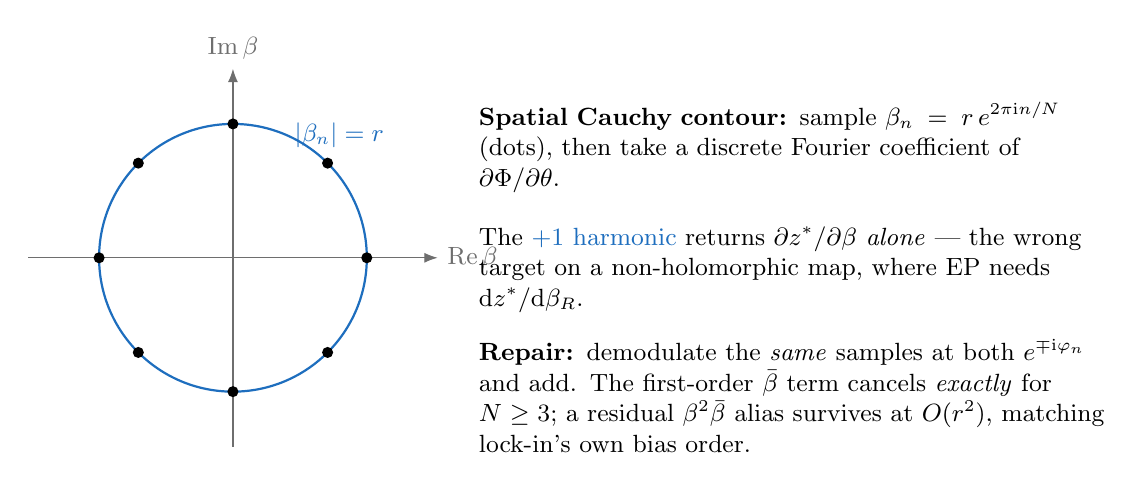
\begin{tikzpicture}[font=\small,>=Latex]
  \draw[->,axisgray] (-2.6,0)--(2.6,0) node[right]{$\Real\beta$};
  \draw[->,axisgray] (0,-2.4)--(0,2.4) node[above]{$\Imag\beta$};
  \draw[holo,thick] (0,0) circle (1.7);
  \node[holo] at (1.35,1.55) {$|\beta_n|=r$};
  \foreach \k in {0,...,7}{
    \pgfmathsetmacro\ang{\k*45}
    \fill[black] (\ang:1.7) circle (2pt);
  }
  \node[anchor=west,align=left,text width=8.0cm] at (3.0,1.4)
    {\textbf{Spatial Cauchy contour:} sample
     $\beta_n=r\,e^{2\pi\im n/N}$ (dots), then take a discrete Fourier
     coefficient of $\partial\Phi/\partial\theta$.};
  \node[anchor=west,align=left,text width=8.0cm] at (3.0,-0.15)
    {The \textcolor{holo}{$+1$ harmonic} returns
     $\partial z^*/\partial\beta$ \emph{alone} --- the wrong target on
     a non-holomorphic map, where EP needs
     $\dd z^*/\dd\beta_R$.};
  \node[anchor=west,align=left,text width=8.0cm] at (3.0,-1.75)
    {\textbf{Repair:} demodulate the \emph{same} samples at both
     $e^{\mp\im\varphi_n}$ and add.  The first-order $\bar\beta$ term
     cancels \emph{exactly} for $N\ge3$; a residual $\beta^2\bar\beta$
     alias survives at $O(r^2)$, matching lock-in's own bias order.};
\end{tikzpicture}
\caption{The spatial Cauchy contour does not so much \emph{fail} as
converge to the wrong quantity.  Its first Fourier coefficient
isolates the holomorphic Wirtinger derivative, which equals the real
directional derivative only when the recurrence is holomorphic.  On
the unit projection recurrence it can be repaired by combining
the $\pm1$ harmonics of the same sampled data --- the spatial analogue
of the two-sideband combination in Figure~\ref{fig:sidebands}.}
\label{fig:contour}
\end{figure}


%======================================================================
\section{Temporal Real-Probe Lock-in}\label{sec:probe}
%======================================================================

\subsection{The probe}

Drive $\beta$ as a real cosine in time at the \emph{probe frequency}
$\omega_p$:
\begin{equation}\label{eq:probe}
  \beta(t)
  \;=\;
  \varepsilon\,\cos(\omega_p t)
  \;=\;
  \frac{\varepsilon}{2}\bigl(e^{\im\omega_p t} + e^{-\im\omega_p t}\bigr),
  \qquad
  \varepsilon \in \R,\ \omega_p > 0.
\end{equation}
The probe stays on the real axis of $\C$ at all times.  When the
network is in its adiabatic regime
(Section~\ref{sec:knobs}) the equilibrium tracks the slowly varying
$\beta(t)$, so the time-dependent state
$\bm{z}(t) \approx \bm{z}^*(\beta(t))$.

\subsection{Linear-response expansion}

Substituting $\beta(t)$ from~\eqref{eq:probe} into~\eqref{eq:dz-wirtinger}
and using $\bar\beta(t) = \beta(t) \in \R$,
\begin{align}
  \bm{z}(t) - \bm{z}^*(0)
  &\;=\;
  \varepsilon\cos(\omega_p t)\,
  \Bigl(
    \frac{\partial\bm{z}^*}{\partial\beta}\bigg|_0
    +
    \frac{\partial\bm{z}^*}{\partial\bar\beta}\bigg|_0
  \Bigr)
  + O(\varepsilon^2) \notag\\
  &\;=\;
  \varepsilon\cos(\omega_p t)\,
  \frac{\dd\bm{z}^*}{\dd\beta_R}\bigg|_0
  + O(\varepsilon^2), \label{eq:linres-state}
\end{align}
where the second line uses~\eqref{eq:real-dir}.  The real-axis
directional derivative $\dd\bm{z}^*/\dd\beta_R$ is what the EP
gradient theorem on real parameters needs.

\subsection{Real vs.\ complex probe}

\begin{figure}[htbp]
\centering
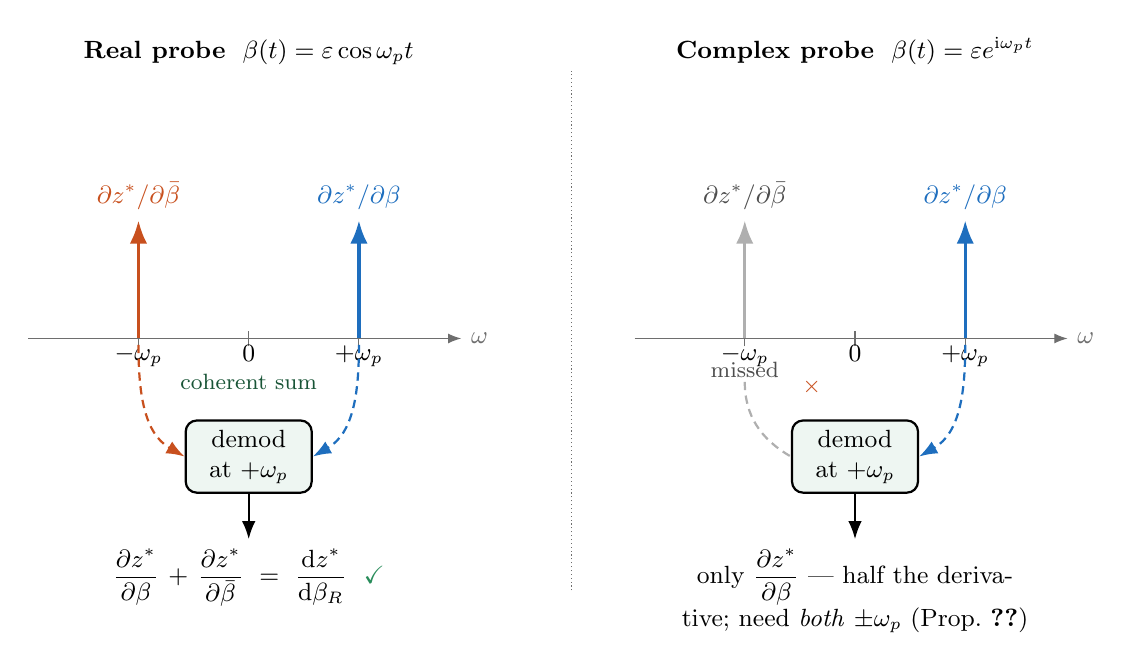
\begin{tikzpicture}[font=\small,>=Latex]
% ================= LEFT: real probe =================
\begin{scope}
  \node[anchor=south,align=center] at (2.5,3.35)
    {\textbf{Real probe}\ \ $\beta(t)=\varepsilon\cos\omega_p t$};
  \draw[->,axisgray] (-0.3,0)--(5.2,0) node[right]{$\omega$};
  \foreach \x/\lab in {1.1/{$-\omega_p$},2.5/{$0$},3.9/{$+\omega_p$}}
    \draw[axisgray] (\x,-0.1)--(\x,0.1) node[below=2pt,black]{\lab};
  % both sidebands live
  \draw[antiholo,very thick,->] (1.1,0)--(1.1,1.5)
     node[above,antiholo]{$\partial z^*/\partial\bar\beta$};
  \draw[holo,very thick,->] (3.9,0)--(3.9,1.5)
     node[above,holo]{$\partial z^*/\partial\beta$};
  % demodulator box
  \node[draw,thick,rounded corners,fill=probeC!8,minimum width=1.6cm,
        minimum height=0.7cm,align=center] (demL) at (2.5,-1.5)
        {demod\\ at $+\omega_p$};
  % BOTH sidebands routed in -> coherent sum
  \draw[antiholo,thick,->,densely dashed] (1.1,-0.08) to[out=-90,in=150] (demL.west);
  \draw[holo,thick,->,densely dashed] (3.9,-0.08) to[out=-90,in=30] (demL.east);
  \node[probeC!60!black,font=\footnotesize] at (2.5,-0.55) {coherent sum};
  \draw[->,thick] (demL.south)--(2.5,-2.55);
  \node[anchor=north,align=center,text width=5cm] at (2.5,-2.55)
    {$\dfrac{\partial z^*}{\partial\beta}+\dfrac{\partial z^*}{\partial\bar\beta}
        =\dfrac{\dd z^*}{\dd\beta_R}$\ \ \textcolor{probeC}{\checkmark}};
\end{scope}
\draw[axisgray,densely dotted] (6.6,-3.2)--(6.6,3.4);
% ================= RIGHT: complex probe =================
\begin{scope}[xshift=7.7cm]
  \node[anchor=south,align=center] at (2.5,3.35)
    {\textbf{Complex probe}\ \ $\beta(t)=\varepsilon e^{\im\omega_p t}$};
  \draw[->,axisgray] (-0.3,0)--(5.2,0) node[right]{$\omega$};
  \foreach \x/\lab in {1.1/{$-\omega_p$},2.5/{$0$},3.9/{$+\omega_p$}}
    \draw[axisgray] (\x,-0.1)--(\x,0.1) node[below=2pt,black]{\lab};
  % -omega_p sideband is greyed: NOT seen by +omega_p demod
  \draw[axisgray!55,very thick,->] (1.1,0)--(1.1,1.5)
     node[above,axisgray!70!black]{$\partial z^*/\partial\bar\beta$};
  \node[axisgray!70!black,font=\footnotesize,anchor=north] at (1.1,-0.18) {missed};
  \draw[holo,very thick,->] (3.9,0)--(3.9,1.5)
     node[above,holo]{$\partial z^*/\partial\beta$};
  % demodulator box
  \node[draw,thick,rounded corners,fill=probeC!8,minimum width=1.6cm,
        minimum height=0.7cm,align=center] (demR) at (2.5,-1.5)
        {demod\\ at $+\omega_p$};
  % only +omega_p routed in; -omega_p route crossed out
  \draw[holo,thick,->,densely dashed] (3.9,-0.08) to[out=-90,in=30] (demR.east);
  \draw[axisgray!55,thick,densely dashed] (1.1,-0.55) to[out=-90,in=150] (demR.west);
  \node[antiholo,font=\footnotesize] at (1.95,-0.62) {$\times$};
  \draw[->,thick] (demR.south)--(2.5,-2.55);
  \node[anchor=north,align=center,text width=5.1cm] at (2.5,-2.55)
    {only $\dfrac{\partial z^*}{\partial\beta}$ — half the derivative;
     need \emph{both} $\pm\omega_p$ (Prop.~\ref{prop:cplx-fail})};
\end{scope}
\end{tikzpicture}
\caption{Why the probe must be \emph{real} in the non-holomorphic
regime.  The state response to a nudge has a holomorphic sideband
($\partial z^*/\partial\beta$, at $+\omega_p$) and an anti-holomorphic
one ($\partial z^*/\partial\bar\beta$, at $-\omega_p$).  \emph{Left:} a
real cosine probe carries both $e^{\pm\im\omega_p t}$, so both
sidebands feed the $+\omega_p$ demodulator and recombine into the
coherent sum $\dd z^*/\dd\beta_R=\partial_\beta+\partial_{\bar\beta}$
— exactly the real-axis directional derivative EP needs.
\emph{Right:} a complex probe places each Wirtinger piece in a
distinct bin, so the $+\omega_p$ demodulator sees only the holomorphic
half and the anti-holomorphic sideband (greyed) is missed; recovering
the full derivative then requires a second demodulation at $-\omega_p$
(Proposition~\ref{prop:cplx-fail}).}
\label{fig:sidebands}
\end{figure}

\begin{proposition}[Probe equivalence in the holomorphic case]
\label{prop:holo-equiv}
If the recurrence is holomorphic in $\beta$ (so
$\partial\bm{z}^*/\partial\bar\beta = 0$) then the real probe
$\beta(t) = \varepsilon\cos(\omega_p t)$ and the complex probe
$\beta(t) = \varepsilon\,e^{\im\omega_p t}$ extract the same linear
coefficient $\partial\bm{z}^*/\partial\beta$ from the first
Fourier coefficient of $\bm{z}(t)$.
\end{proposition}
\begin{proof}
With $\partial/\partial\bar\beta = 0$,~\eqref{eq:dz-wirtinger}
collapses to $\beta\,\partial\bm{z}^*/\partial\beta + O(|\beta|^2)$.
For the real probe the Fourier coefficient at $+\omega_p$ is
$(\varepsilon/2)\partial\bm{z}^*/\partial\beta$; for the complex probe
it is $\varepsilon\,\partial\bm{z}^*/\partial\beta$.  They agree up
to the factor of 2 absorbed in the gradient formula
of Section~\ref{sec:grad}.
\end{proof}

The complex probe is not unusable on a non-holomorphic recurrence, but
single-sideband demodulation at $+\omega_p$ recovers only the
holomorphic half $\partial\bm{z}^*/\partial\beta$ --- the wrong target
for real parameters.  Recovering the full directional derivative
$\dd\bm{z}^*/\dd\beta_R$ then requires \emph{two} demodulation
accumulators, at $+\omega_p$ and $-\omega_p$, and their coherent sum;
the same two-sideband repair extends even to the quadratic Hebbian
observable, despite the sideband mixing introduced by its conjugated
factor.  The precise statement and proof are collected as
Proposition~\ref{prop:cplx-fail} in Appendix~\ref{app:sidebands}.

\begin{corollary}[Why the real probe]\label{cor:why-real}
On a non-holomorphic recurrence (the phasor-EP regime with
unit projection), the real probe excites both Wirtinger
sidebands coherently, so its $+\omega_p$ Fourier coefficient already
contains the full $\dd\bm{z}^*/\dd\beta_R$ directional derivative —
exactly the quantity finite-difference EP on real parameters would
estimate — in a \emph{single} demodulation.  A complex probe recovers
the same quantity only by coherently combining two sideband
demodulations (Proposition~\ref{prop:cplx-fail}); the real probe's
advantage is operational, not one of possibility.
\end{corollary}

%======================================================================
\section{Lock-in Demodulation}\label{sec:demod}
%======================================================================

\subsection{Continuous-time formula}

The Hebbian outer product is the parameter-gradient quantity of
interest.  For weight matrix $W_\ell$ at layer $\ell$, define the
time-dependent Hebbian observable
\begin{equation}\label{eq:hebb-obs}
  H_\ell(t)
  \;=\;
  \bm{z}_\ell(t)\,\bm{z}_{\ell-1}(t)^H,
\end{equation}
which evaluates to $\bm{z}_\ell^*(\beta(t))\,\bm{z}_{\ell-1}^*(\beta(t))^H$
in the adiabatic regime.  The lock-in coefficient at $+\omega_p$ over
an integer number of probe cycles $T_\text{int} = 2\pi N_c/\omega_p$
($N_c \in \mathbb{Z}_{>0}$) is
\begin{equation}\label{eq:lockin-cont}
  H_\ell^{+}
  \;=\;
  \frac{1}{T_\text{int}}
  \int_0^{T_\text{int}}
  \bigl(H_\ell(t) - H_\ell^{\text{DC}}\bigr)\,
  e^{-\im\omega_p t}\,\dd t,
\end{equation}
where $H_\ell^{\text{DC}} = H_\ell(\bm{z}^*(0))$ is the free-equilibrium
Hebbian.  Note that over \emph{exactly} integer cycles any constant
integrates against $e^{-\im\omega_p t}$ to zero, so this subtraction
is not a correctness requirement; it is a leakage/variance-reduction
measure that matters when $T_\text{int}$ only approximately spans
integer cycles (cf.\ Section~\ref{sec:knobs}) or when the DC term is
large compared with the $O(\varepsilon)$ signal in finite arithmetic.

\subsection{Sideband bookkeeping}

Expanding the integrand using~\eqref{eq:linres-state} on $\bm{z}_\ell$ and
$\bm{z}_{\ell-1}$ separately,
\begin{equation}\label{eq:H-expand}
  H_\ell(t) - H_\ell^{\text{DC}}
  \;=\;
  \varepsilon\cos(\omega_p t)\,
  \frac{\dd H_\ell^*}{\dd\beta_R}\bigg|_0
  \;+\;
  O(\varepsilon^2),
\end{equation}
with $H_\ell^* = \bm{z}_\ell^*\bm{z}_{\ell-1}^{*\,H}$.  Demodulating,
\begin{equation}\label{eq:demod-step}
  H_\ell^{+}
  \;=\;
  \varepsilon\cdot\frac{1}{T_\text{int}}\!\int_0^{T_\text{int}}
  \cos(\omega_p t)\,e^{-\im\omega_p t}\,\dd t
  \cdot \frac{\dd H_\ell^*}{\dd\beta_R}\bigg|_0
  + O(\varepsilon^2).
\end{equation}
Over integer cycles
$(1/T_\text{int})\!\int_0^{T_\text{int}}\!\cos(\omega_p t)\,e^{-\im\omega_p t}\dd t
 = \tfrac{1}{2}$.  Moreover, the $O(\varepsilon^2)$ term
of~\eqref{eq:H-expand} carries
$\cos^2(\omega_p t) = \tfrac12\bigl(1 + \cos 2\omega_p t\bigr)$, whose
spectral content lies at DC and $\pm2\omega_p$ and is therefore
annihilated by the $+\omega_p$ demodulation over integer cycles.  The
first surviving contamination comes from the $\cos^3$ term at
$O(\varepsilon^3)$:
\begin{equation}\label{eq:HpHebbian}
  H_\ell^{+}
  \;=\;
  \tfrac{\varepsilon}{2}\,
  \frac{\dd H_\ell^*}{\dd\beta_R}\bigg|_0
  \;+\;
  O(\varepsilon^3).
\end{equation}
This even-order rejection is the same mechanism exploited by
oscillatory nudging in holomorphic EP (Laborieux--Zenke).

%======================================================================
\section{Gradient Extraction Formula}\label{sec:grad}
%======================================================================

\subsection{Main result}

Combining the EP gradient theorem~\eqref{eq:static-ep}, the chain
rule through the equilibrium, the linear-response
expansion~\eqref{eq:linres-state}, and the demodulation
formula~\eqref{eq:HpHebbian}, and remembering the sign flip from
$\Phi = E - \beta\mathcal{C}$ (the loss enters with a minus sign):

\begin{theorem}[Lock-in EP gradient]\label{thm:lockin-grad}
For the phasor energy~\eqref{eq:energy} with the real-probe
$\beta(t) = \varepsilon\cos(\omega_p t)$ in the adiabatic regime
(Section~\ref{sec:knobs}), the loss gradient with respect to a real
weight matrix $W_\ell$ is
\begin{equation}\label{eq:main-grad}
  \boxed{
  \frac{\dd\mathcal{L}}{\dd W_\ell}
  \;=\;
  -\frac{2}{\varepsilon}\,\Real\bigl(H_\ell^{+}\bigr)
  \;+\; O(\varepsilon^2),
  }
\end{equation}
where $H_\ell^{+}$ is the DC-subtracted lock-in
coefficient~\eqref{eq:lockin-cont}.  The factor of 2 cancels the
$\tfrac{1}{2}$ in~\eqref{eq:HpHebbian}; the minus sign converts
$\partial\Phi/\partial W$ to $\dd\mathcal{L}/\dd W$ for gradient
descent; the real part projects out the imaginary residual that would
appear from incomplete cycle cancellation or higher-order Wirtinger
mixing.  The bias is $O(\varepsilon^2)$ rather than $O(\varepsilon)$
by the even-order rejection of~\eqref{eq:HpHebbian}: the quadratic
response is invisible at $+\omega_p$, and the leading contamination is
cubic.  The prefactor $2/\varepsilon$ matches the real-parameter nudge
convention~\eqref{eq:drift-is-2grad} and neglects the adiabatic phase
lag; at finite $\omega_p$ the estimate is additionally attenuated by
$\cos\phi$ with $\phi\sim\omega_p/R_\text{relax}$ (see
Section~\ref{sec:knobs}).
\end{theorem}

\subsection{Discrete-time implementation}

In the discrete settling loop with time step $\dt$, the probe
$\beta[n] = \varepsilon\cos(\omega_p\,n\,\dt)$ for
$n = 1,\dots,T_\text{lockin}$ with
$T_\text{lockin} = N_c \cdot (2\pi/(\omega_p\dt))$
(integer cycles).  The discrete lock-in accumulator is
\begin{equation}\label{eq:disc-acc}
  \tilde H_\ell^{+}
  \;=\;
  \sum_{n=1}^{T_\text{lockin}}
    \bigl(\bm{z}_\ell^{(n)} (\bm{z}_{\ell-1}^{(n)})^H - H_\ell^{\text{DC}}\bigr)
    \cdot e^{-\im\omega_p n \dt},
\end{equation}
and the gradient~\eqref{eq:main-grad} becomes
\begin{equation}\label{eq:disc-grad}
  \widehat{\frac{\dd\mathcal{L}}{\dd W_\ell}}
  \;=\;
  -\frac{2}{T_\text{lockin}\,\varepsilon}\,\Real\bigl(\tilde H_\ell^{+}\bigr).
\end{equation}
This is the discrete estimator used in practice; it is a drop-in
replacement for the two static free/nudged Hebbian differences of
vanilla EP, accumulated over the lock-in window instead.

\subsection{Warm-up}

\begin{figure}[htbp]
\centering
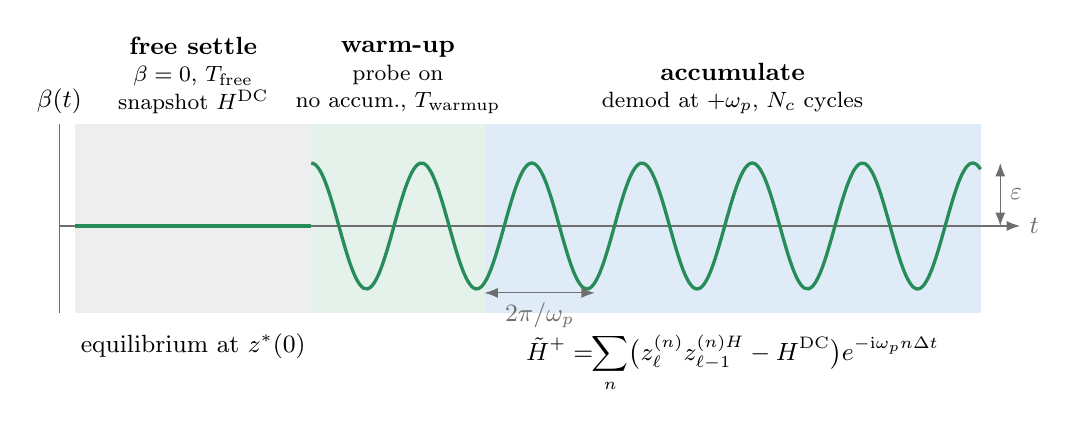
\begin{tikzpicture}[font=\small,>=Latex]
  \def\yb{0}
  \def\A{0.8}
  \fill[axisgray!12]  (0,\yb-1.1) rectangle (3,\yb+1.3);
  \fill[probeC!12]    (3,\yb-1.1) rectangle (5.2,\yb+1.3);
  \fill[holo!14]      (5.2,\yb-1.1) rectangle (11.5,\yb+1.3);
  \draw[->,axisgray] (-0.2,\yb)--(12.0,\yb) node[right]{$t$};
  \draw[axisgray] (-0.2,\yb-1.1)--(-0.2,\yb+1.3) node[above,black]{$\beta(t)$};
  \draw[probeC,very thick] (0,\yb)--(3,\yb);
  \draw[probeC,very thick,domain=3:11.5,samples=180,smooth]
     plot (\x,{\yb+\A*cos(360*(\x-3)/1.4)});
  \draw[<->,axisgray] (11.75,\yb)--(11.75,\yb+\A) node[midway,right]{$\varepsilon$};
  \draw[<->,axisgray] (5.2,\yb-0.85)--(6.6,\yb-0.85)
     node[midway,below]{$2\pi/\omega_p$};
  \node[align=center,anchor=south] at (1.5,\yb+1.3)
    {\textbf{free settle}\\[-1pt]\footnotesize $\beta=0$,\ $T_\text{free}$\\[-1pt]
     \footnotesize snapshot $H^{\text{DC}}$};
  \node[align=center,anchor=south] at (4.1,\yb+1.3)
    {\textbf{warm-up}\\[-1pt]\footnotesize probe on\\[-1pt]
     \footnotesize no accum., $T_\text{warmup}$};
  \node[align=center,anchor=south] at (8.35,\yb+1.3)
    {\textbf{accumulate}\\[-1pt]\footnotesize demod at $+\omega_p$,\ $N_c$ cycles};
  \node[anchor=north,align=center] at (8.35,\yb-1.25)
    {$\displaystyle \tilde H^{+}=\!\!\sum_{n}\bigl(z_\ell^{(n)}z_{\ell-1}^{(n)H}-H^{\text{DC}}\bigr)e^{-\im\omega_p n\Delta t}$};
  \node[anchor=north] at (1.5,\yb-1.25){equilibrium at $z^*(0)$};
\end{tikzpicture}
\caption{The three-phase lock-in schedule as a function of settling
time.  During the \emph{free settle} the nudge is off and the network
reaches $z^*(0)$, whose Hebbian $H^{\text{DC}}$ is stored for DC
subtraction.  The probe $\beta(t)=\varepsilon\cos\omega_p t$ is then
switched on; the \emph{warm-up} discards $T_\text{warmup}$ so the
equilibrium can lock onto the modulation, and only the
\emph{accumulate} window (an integer number $N_c$ of probe periods) is
demodulated at $+\omega_p$ into $\tilde H^{+}$.  If the warm-up and
accumulation loops each run their own step counter, the probe clock
resets at the warm-up/accumulate boundary
(Section~\ref{sec:grad}).}
\label{fig:timeline}
\end{figure}

Before the lock-in accumulator runs, the network settles to
$\bm{z}^*(0)$ at $\beta=0$ (the \emph{free phase}, $T_\text{free}$
steps) so $H_\ell^{\text{DC}}$ is well-defined.  Then $\beta(t)$ is
switched on for $T_\text{warmup} = N_\text{warmup}\cdot(2\pi/(\omega_p\dt))$
steps with no accumulation, to let the equilibrium catch up to the
modulation.  Only then is the accumulator~\eqref{eq:disc-acc}
populated.  Skipping warm-up leaks transient
$\bm{z}(t)-\bm{z}^*(0)$ into the first cycles' integrand and biases
the gradient toward whatever direction the transient happened to
take.  One implementation subtlety: the probe clock \emph{resets}
between the warm-up and accumulation loops (each runs
$t = 1,\dots,T$ with its own $t$), so probe/demodulator phase
continuity across the boundary relies on $T_\text{warmup}$ spanning
integer periods — which it does only up to the same
$\mathrm{round}(2\pi/(\omega_p\dt))$ residual discussed in
Section~\ref{sec:knobs}.  The resulting phase jump is
$O\bigl(N_\text{warmup}\,|\,2\pi - \omega_p\dt\cdot
\mathrm{round}(2\pi/(\omega_p\dt))\,|\bigr)$ per boundary (about
$4\times10^{-3}$ rad at the default knobs) and injects a
correspondingly small transient into the first accumulated cycle.

%======================================================================
\section{Bias Gradient}\label{sec:bias}
%======================================================================

When the layer has a complex bias $\bm{b}_\ell = \bm{b}_\ell^R + \im\bm{b}_\ell^I$,
the bias enters the energy through the coupling term as
$\Real\langle W_\ell\bm{z}_{\ell-1} + \bm{b}_\ell, \bm{z}_\ell\rangle$.
The Hebbian observable for the bias is simply
$\bm{z}_\ell(t)$ (not an outer product), and the lock-in coefficient
is
\begin{equation}\label{eq:bias-acc}
  \tilde H_{\ell,b}^{+}
  \;=\;
  \sum_{n=1}^{T_\text{lockin}}
    \bigl(\bm{z}_\ell^{(n)} - \bm{z}_\ell^{(0)}\bigr)\,
    e^{-\im\omega_p n\dt}.
\end{equation}
The real and imaginary parts of $\tilde H_{\ell,b}^{+}$ correspond
to the gradients with respect to $\bm{b}_\ell^R$ and $\bm{b}_\ell^I$
independently:
\begin{equation}\label{eq:bias-grad}
  \widehat{\frac{\dd\mathcal{L}}{\dd \bm{b}_\ell^R}}
  \;=\;
  -\frac{2}{T_\text{lockin}\,\varepsilon}\,\Real\bigl(\tilde H_{\ell,b}^{+}\bigr),
  \qquad
  \widehat{\frac{\dd\mathcal{L}}{\dd \bm{b}_\ell^I}}
  \;=\;
  -\frac{2}{T_\text{lockin}\,\varepsilon}\,\Imag\bigl(\tilde H_{\ell,b}^{+}\bigr).
\end{equation}
Packaging $\bm{z}_\ell^{(n)}$ directly as a complex number lets a
single demodulation accumulator handle both the real and imaginary bias
parts at once.

%======================================================================
\section{Accuracy Knobs and Failure Modes}\label{sec:knobs}
%======================================================================

\subsection{Three knobs}

\begin{center}
\small
\begin{tabular}{lll}
\toprule
\textbf{Knob} & \textbf{Controls} & \textbf{Failure modes} \\
\midrule
$\varepsilon$ & Linearity of the response &
  Too small: noise floor of $H_\ell^{+}$. \\
  & & Too large: $O(\varepsilon^2)$ nonlinearity bias. \\
$\omega_p$ & Separation from natural $\bm{\omega}$; adiabaticity &
  Too low: probe cycle longer than budget. \\
  & & Too high: non-adiabatic, system can't track $\bm{z}^*(\beta(t))$. \\
$N_c$ (cycles) & Demodulator selectivity &
  Too small: aliasing from imperfectly cancelled \\
  & & ~~harmonics. \\
  & & Too large: linear cost in settling time. \\
\bottomrule
\end{tabular}
\end{center}

\subsection{Stability constraints}

\begin{figure}[htbp]
\centering
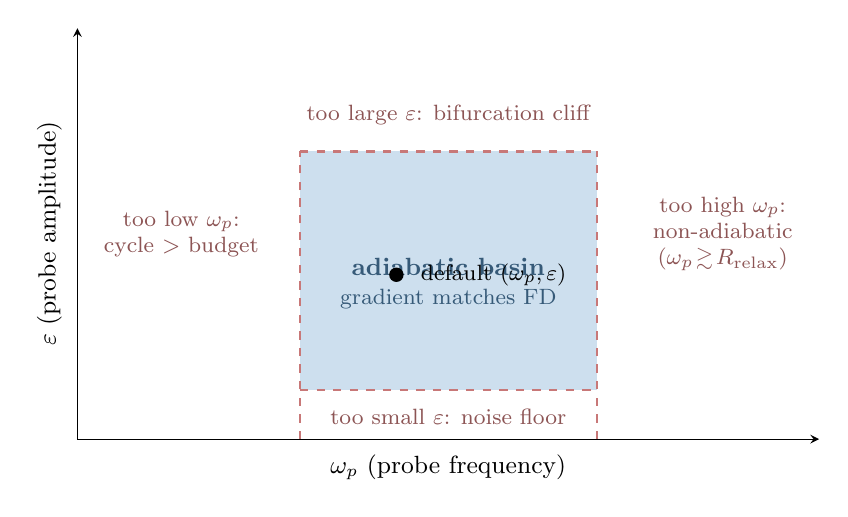
\begin{tikzpicture}[font=\small,>=Latex]
\begin{axis}[
   width=11cm,height=6.8cm,
   xlabel={$\omega_p$ (probe frequency)},
   ylabel={$\varepsilon$ (probe amplitude)},
   xmin=0,xmax=10,ymin=0,ymax=10,
   xtick=\empty,ytick=\empty,
   axis lines=left,
   clip=false,
]
  \fill[basinC!30] (axis cs:3,1.2) rectangle (axis cs:7,7.0);
  \node[basinC!60!black] at (axis cs:5,4.2) {\textbf{adiabatic basin}};
  \node[basinC!60!black,font=\footnotesize] at (axis cs:5,3.4)
     {gradient matches FD};
  \fill[black] (axis cs:4.3,4.0) circle (2.6pt);
  \node[anchor=west,font=\footnotesize] at (axis cs:4.5,4.0)
     {default $(\omega_p,\varepsilon)$};
  \node[badC!70!black,align=center,font=\footnotesize] at (axis cs:1.4,5){too low $\omega_p$:\\ cycle $>$ budget};
  \node[badC!70!black,align=center,font=\footnotesize] at (axis cs:8.7,5){too high $\omega_p$:\\ non-adiabatic\\ ($\omega_p\!\gtrsim\!R_\text{relax}$)};
  \node[badC!70!black,align=center,font=\footnotesize] at (axis cs:5,7.9){too large $\varepsilon$: bifurcation cliff};
  \node[badC!70!black,align=center,font=\footnotesize] at (axis cs:5,0.55){too small $\varepsilon$: noise floor};
  \draw[badC,dashed,thick] (axis cs:3,0)--(axis cs:3,7.0);
  \draw[badC,dashed,thick] (axis cs:7,0)--(axis cs:7,7.0);
  \draw[badC,dashed,thick] (axis cs:3,7.0)--(axis cs:7,7.0);
  \draw[badC,dashed,thick] (axis cs:3,1.2)--(axis cs:7,1.2);
\end{axis}
\end{tikzpicture}
\caption{The operating region in the $(\omega_p,\varepsilon)$ plane.
The two frequency bounds come from~\eqref{eq:freq-sep}
and~\eqref{eq:adiabatic}: $\omega_p$ must be high enough to fit whole
cycles in the settling budget yet well below the relaxation rate
$R_\text{relax}$ for adiabatic following.  The amplitude bounds are
the $H^{+}$ noise floor below and the bifurcation cliff of
Section~\ref{sec:knobs} above.  The basin is wide --- roughly a decade
in each knob --- with the default $(\omega_p,\varepsilon)=(0.05,0.05)$
sitting comfortably inside.}
\label{fig:basin}
\end{figure}

The probe oscillation must lie outside every channel's natural
oscillator bandwidth and inside the network's relaxation rate:
\begin{align}
  |\omega_p - \omega_{\ell,c}| &> |\lambda_{\ell,c}|
  \qquad \text{for every channel } (\ell, c),
  \label{eq:freq-sep}\\
  \omega_p &\ll
  R_\text{relax}
  \;\approx\;
  \min_{\ell,c}|\lambda_{\ell,c}| + \|W\|_\text{op}.
  \label{eq:adiabatic}
\end{align}
\eqref{eq:freq-sep} is the \emph{frequency-separation} condition:
the probe response should not be confused with the natural channel
oscillation. \eqref{eq:adiabatic} is the \emph{adiabatic-following}
condition: the probe period $2\pi/\omega_p$ should be much longer
than the network's settling time scale so $\bm{z}(t)$ remains close
to the instantaneous equilibrium $\bm{z}^*(\beta(t))$.

\paragraph{Adiabatic lag is a systematic error, not only a validity
condition.}
At finite $\omega_p$ the state tracks $\bm{z}^*(\beta(t))$ with a
delay: to first order in $\omega_p/R_\text{relax}$, the linear
response is $\varepsilon\,|\chi(\omega_p)|\cos(\omega_p t - \phi)$
with lag $\phi \sim \omega_p/R_\text{relax}$.  The demodulated
coefficient then acquires a factor $e^{-\im\phi}$, so taking
$\Real(H_\ell^{+})$ in~\eqref{eq:main-grad} attenuates the gradient by
$\cos\phi$ and folds a fraction $\sin\phi$ of the quadrature
component into the estimate.  Condition~\eqref{eq:adiabatic} bounds
$\phi$ but does not remove it.  The standard lock-in remedy is
cheap: accumulate both quadratures and rotate by a reference phase
calibrated once (\eg\ against a channel or a finite-difference probe
whose response is known), rather than assuming $\phi = 0$.

\subsection{Integer-cycle requirement}

The accumulator~\eqref{eq:disc-acc} must run for an integer number of
probe periods.  Non-integer cycles leak even-harmonic content
(notably the DC component of $\cos^2(\omega_p t)$) into the
$+\omega_p$ coefficient, biasing the gradient.  Setting
$T_\text{lockin} = N_c \cdot \mathrm{round}(2\pi/(\omega_p\dt))$ with
$N_c \ge 2$ is the practical recipe; tighter integer alignment
requires $\omega_p\dt$ to divide $2\pi$ exactly, which is rarely
worth engineering.  Alternatively, applying a tapered window (Hann or
flat-top) to the accumulator~\eqref{eq:disc-acc} suppresses the
leakage of non-integer cycles at a small cost in effective
bandwidth, relaxing the alignment requirement entirely — the
standard trade in lock-in and FFT practice.

\subsection{Bifurcation cliff}

The linear-response expansion~\eqref{eq:linres-state} is local
around $\bm{z}^*(0)$.  If $\varepsilon$ is large enough that
$\beta(t)$ pushes the network through a saddle-node or pitchfork
bifurcation of the equilibrium map, $\bm{z}^*(\beta(t))$ jumps
discontinuously and the lock-in estimator becomes meaningless.  The
amplitude at which this happens is the \emph{basin radius} of
$\bm{z}^*(0)$ in the $\beta$-direction and depends on the network
state; in practice $\varepsilon \in [0.01, 0.1]$ is well inside the
basin for the demonstrated networks.

%======================================================================
\section{Relationships to Other EP Variants}\label{sec:rel}
%======================================================================

\subsection{Holomorphic limit}

\begin{corollary}[Lock-in $\leftrightarrow$ spatial Cauchy contour]
\label{cor:holo-limit}
If the recurrence is holomorphic in $\beta$ (no unit projection,
holomorphic $\sigma$, bilinear inner product as in the companion
holomorphic-EP derivation), the lock-in
formula~\eqref{eq:main-grad} agrees with the spatial Cauchy
contour formula of holomorphic EP up to discretization.  In this
regime both probes (real and complex) extract the same gradient
(Proposition~\ref{prop:holo-equiv}) and the choice between them is
purely operational.
\end{corollary}

\subsection{Small-$\varepsilon$ limit}

\begin{corollary}[Lock-in $\leftrightarrow$ static EP]
\label{cor:static-limit}
At $N_c = 1$, $\omega_p\dt \to 0$, the
accumulator~\eqref{eq:disc-acc} reduces to a single Hebbian
difference $H_\ell(t_+) - H_\ell(t_-)$ with $t_\pm$ at the cosine
peaks $\pm\varepsilon$.  This is, up to a sign, the \emph{symmetric}
(centered) two-point estimator
$\bigl(H_\ell(+\varepsilon)-H_\ell(-\varepsilon)\bigr)/(2\varepsilon)$
— the centered variant of the one-sided two-phase estimator of
static EP~\eqref{eq:static-ep}, whose even-order cancellation is the
static shadow of the $O(\varepsilon^2)$ bias
of~\eqref{eq:main-grad}.  Lock-in is the time-multiplexed
generalization that gains noise rejection from $N_c > 1$ at fixed
$\varepsilon$.
\end{corollary}

\subsection{Frequency multiplexing}

Because each parameter direction's gradient lives at a chosen
$\omega_p$, several gradient extractions can run simultaneously
with distinct probe frequencies $\omega_p^{(k)}$ in the same
settle.  Each accumulator demodulates at its own
$\omega_p^{(k)}$ and the orthogonality of distinct Fourier
components separates them.  The frequency-separation
condition~\eqref{eq:freq-sep} must hold for every $\omega_p^{(k)}$
pair and against every natural $\omega_{\ell,c}$.  This is
\emph{frequency-domain gradient parallelism}, not currently
implemented but a natural extension of the present formula.

\emph{Caveat (intermodulation).}  Because the Hebbian observable is
quadratic in the state, two probes at $\omega_p^{(1)},\omega_p^{(2)}$
generate second-order products at $\omega_p^{(1)}\pm\omega_p^{(2)}$
(and higher-order intermodulation at $O(\varepsilon^2)$ and beyond).
Pairwise separation of the probe frequencies and separation from
every natural $\omega_{\ell,c}$ is therefore \emph{not} sufficient:
the frequency plan must also keep all sum and difference frequencies
off every demodulation bin, as in standard multi-tone lock-in
practice.

%======================================================================
\section{Practical Defaults and Training}\label{sec:practical}
%======================================================================

A useful starting operating point sits deep in the adiabatic basin of
Section~\ref{sec:knobs}: a small amplitude $\varepsilon\approx0.05$, a
probe frequency $\omega_p$ well below the relaxation rate
$R_\text{relax}$ but high enough to fit several whole cycles in the
settling budget, a handful of demodulation cycles ($N_c\sim8$), one or
two warm-up cycles, and a free settle long enough to reach $\bm{z}^*(0)$.
Around such a point the lock-in gradient typically matches a
finite-difference oracle to a few percent across roughly a decade in
each knob, with the failure modes as tabulated in
Section~\ref{sec:knobs}.

When training all the way to low loss, it helps to reduce the amplitude
(\eg\ to $\varepsilon\approx0.01$): the smaller drive trades a slightly
higher noise floor for a smaller $O(\varepsilon^2)$ nonlinearity bias,
which dominates once the loss approaches zero.  Because the lock-in
gradient carries a few-percent directional noise that the noise-free
static estimator does not, a proportionally larger number of training
epochs compensates.  As an end-to-end sanity check, the two- and
four-corner XOR problems are learned by both the static and the lock-in
estimator provided a bias term is enabled and the input and target use
a consistent $\{0^\circ,90^\circ\}$ phase encoding; disabling the bias is
a useful counter-example that fails to converge.

%======================================================================
\section{Summary}\label{sec:summary}
%======================================================================

\begin{enumerate}
\item Phasor networks in the unit-circle regime use a unit-projection
  nonlinearity that is \textbf{not holomorphic} in the state $\bm{z}$
  and therefore not holomorphic in the nudge $\beta$.  The spatial
  Cauchy contour of holomorphic EP annihilates the anti-holomorphic
  sideband exactly at first order for $N\ge3$, but converges to the
  \emph{wrong target} — $\partial\bm{z}^*/\partial\beta$ rather than
  $\dd/\dd\beta_R$ — and retains an aliased $O(r^2)$ mixed-term bias
  (Appendix~\ref{app:sidebands}).  It can be repaired by two-sideband
  demodulation, at the cost of a second accumulator and coherent
  combination.

\item On the projected (torus-constrained) equilibrium, the EP
  gradient theorem holds because the residual energy gradient at a
  projected fixed point is radial and hence invisible to tangential
  variations (Lemma~\ref{lem:stationarity}).  In the benchmarked
  configuration the drift is exactly $2\,\partial\Phi/\partial\bar{\bm{z}}$
  \eqref{eq:drift-is-2grad} under the real-parameter nudge convention
  $\mathrm{nudge}=(\beta/d_L)\bm{y}$, so the lemma applies with no
  caveat; the variant that folds in the oscillator self-force adds a
  non-variational rotation $\tfrac12\im\bm{\omega}\odot\bm{z}$, which
  requires the rotating-frame reduction (uniform $\bm{\omega}$) before
  the theorem applies (Appendix~\ref{app:stationarity}).

\item Driving $\beta$ as a \textbf{real cosine in time}
  $\beta(t) = \varepsilon\cos(\omega_p t)$ excites both Wirtinger
  sidebands coherently.  Demodulating at $+\omega_p$ over integer
  cycles extracts $\tfrac{\varepsilon}{2}\,\dd H_\ell^*/\dd\beta_R$ —
  the real-axis directional derivative, which is exactly the quantity
  finite-difference EP on real parameters needs — in a single
  accumulator (Corollary~\ref{cor:why-real}).

\item The complex probe $\beta(t) = \varepsilon\,e^{\im\omega_p t}$
  with single-sideband demodulation gives only the holomorphic
  Wirtinger half; combining both sidebands repairs it, including for
  the quadratic Hebbian observable
  (Proposition~\ref{prop:cplx-fail}).  It is directly correct in the
  holomorphic regime (Proposition~\ref{prop:holo-equiv}); the real
  probe's advantage in the unit-circle regime is operational.

\item The full gradient formula (Theorem~\ref{thm:lockin-grad})
  has a factor of $2/\varepsilon$, a minus sign from the EP energy
  convention $\Phi = E - \beta\mathcal{C}$, and the real part to
  project out residual imaginary contributions.  Its bias is
  $O(\varepsilon^2)$ by even-order rejection ($\cos^2$ content lies
  at DC and $2\omega_p$ and is invisible at $+\omega_p$); adiabatic
  phase lag adds a systematic $\cos\phi$ attenuation,
  $\phi\sim\omega_p/R_\text{relax}$, removable by two-quadrature
  accumulation with a calibrated reference phase.

\item Three knobs $(\varepsilon, \omega_p, N_c)$ control three
  failure modes; the adiabatic basin in $(\varepsilon, \omega_p)$
  is wide and easy to land in, with $\varepsilon \in [0.01, 0.1]$
  and $\omega_p \ll R_\text{relax}$ as the practical defaults.

\item Lock-in reduces to the spatial Cauchy contour in the
  holomorphic limit (Corollary~\ref{cor:holo-limit}) and to
  two-phase static EP at $N_c = 1$
  (Corollary~\ref{cor:static-limit}).  Beyond the regimes
  recovered by those limits, it generalizes naturally to
  \textbf{frequency multiplexing} across parameter directions,
  subject to an intermodulation-aware frequency plan
  (Section~\ref{sec:rel}).

\item Algorithmically, lock-in EP keeps the two-phase skeleton of
  vanilla EP: a free settle to $\bm{z}^*(0)$, a driven settle under the
  cosine probe, and a single Hebbian accumulator read out
  by~\eqref{eq:disc-grad} in place of the free/nudged difference.  The
  heavier arguments --- the drift decomposition and stationarity proof,
  and the two-sideband algebra --- are collected in
  Appendices~\ref{app:stationarity}--\ref{app:sidebands}.
\end{enumerate}

\section*{References}

\begin{itemize}
\item Scellier, B.\ \& Bengio, Y.\ (2017). ``Equilibrium
  Propagation: Bridging the Gap Between Energy-Based Models and
  Backpropagation.'' \emph{Frontiers in Computational Neuroscience}.
\item Laborieux, A.\ \& Zenke, F.\ (2022). ``Holomorphic Equilibrium
  Propagation Computes Exact Gradients Through Finite Size
  Oscillations.'' NeurIPS 2022. arXiv:2209.00530.  (The spatial
  Cauchy contour technique is adapted from this paper; it is treated in
  the companion holomorphic-EP derivation.)
\item Wirtinger, W.\ (1927). ``Zur formalen Theorie der Funktionen
  von mehr komplexen Veränderlichen.'' \emph{Mathematische Annalen}
  97, 357--375.
\end{itemize}

\appendix

%======================================================================
\section{Drift Decomposition and Stationarity}\label{app:stationarity}
%======================================================================

This appendix expands the two claims deferred from
Section~\ref{sec:phasor-ep}: that the settling drift is (twice) the
Wirtinger gradient of the energy in the benchmarked configuration, and
that the projected equilibrium is stationary up to a radial residual.

\subsection*{The drift versus the Wirtinger gradient}

The Wirtinger gradient of the energy~\eqref{eq:energy} is
\begin{equation}\label{eq:true-grad}
  \frac{\partial\Phi}{\partial\bar{\bm{z}}_\ell}
  \;=\;
  \tfrac{1}{2}\Lambda_\ell\bm{z}_\ell
  \;+\;
  \tfrac{1}{2}W_\ell\bm{z}_{\ell-1}
  \;+\;
  \tfrac{1}{2}W_{\ell+1}^{\!\top}\bm{z}_{\ell+1}
  \;-\;
  \beta\,\delta_{\ell L}\,
  \frac{\partial\mathcal{C}}{\partial\bar{\bm{z}}_L},
  \qquad \Lambda_\ell = \diag(\bm{\lambda}_\ell),
\end{equation}
because $\tfrac12\Real\langle\bm{z},K\bm{z}\rangle
= \tfrac12\sum_j \lambda_j |z_j|^2$ depends only on $\Real K$ (on the
torus it is moreover \emph{constant}, so the self-energy does no work
in the constrained dynamics; any radial term $\bm{\mu}\odot\bm{z}$ with
real $\bm{\mu}$ is annihilated by the projection anyway), and
$\partial_{\bar z}\,\Real\langle\bm{u},\bm{z}\rangle = \tfrac12\bm{u}$.
The implemented drift~\eqref{eq:settle-grad} differs
from~\eqref{eq:true-grad} in two ways.

\paragraph{(i) Rotational component.}
When the oscillator self-force is folded into the drift, the term
$\tfrac12\,\im\,\bm{\omega}_\ell\odot\bm{z}_\ell$ appears; it is not the
gradient of any real energy.  It is purely tangential to the torus
($\Real(\bar z_j\cdot\im\omega_j z_j)=0$), so at a fixed point the
tangential part of the true gradient must cancel it --- meaning
$\bm{z}^*$ is \emph{not} a constrained critical point of $\Phi$ when
$\bm{\omega}\ne\bm{0}$, and the envelope argument of
Lemma~\ref{lem:stationarity} does not directly apply.  For uniform
$\omega_{\ell,c}\equiv\omega$ the rotation is removed exactly by the
rotating-frame substitution $\bm{z}\mapsto e^{\im\omega t}\bm{w}$: the
Hermitian couplings $\Real\langle W\bm{z}_{\ell-1},\bm{z}_\ell\rangle$
are invariant under a global phase, provided the target $\bm{y}$ is
defined in the rotating frame.  For non-uniform $\bm{\omega}$ no such
global frame exists.  In the default and benchmarked configuration the
$K$ term is dropped from the drift entirely, so $\bm{\lambda}$ and
$\bm{\omega}$ are absent and the issue is moot; the rotating-frame
construction is the path to extending the derivation to the self-force
variant.

\paragraph{(ii) Term-wise factors.}
With the $K$ term dropped and the cost drift
$-2\beta\,\partial\mathcal{C}/\partial\bar{\bm{z}}_L$, the drift
satisfies \emph{exactly}
\begin{equation}\label{eq:drift-is-2grad}
  \bm{g}_\ell \;=\; 2\,\frac{\partial\Phi}{\partial\bar{\bm{z}}_\ell},
\end{equation}
the steepest-descent direction of a real function of complex variables
($\nabla = 2\,\partial/\partial\bar z$).  The overall factor of $2$
rescales the flow without moving its fixed points, and the
$\beta$-scaling of the nudge matches the $\beta$ that the EP
estimator~\eqref{eq:static-ep} divides by, so the constants of
Theorem~\ref{thm:lockin-grad} are as stated.  Had the cost drift
carried the na\"ive Wirtinger factor
$-\beta\,\partial\mathcal{C}/\partial\bar{\bm{z}}_L$ instead, the
effective nudge would be $\beta/2$ and every EP prefactor would double.
This is the subtle convention point behind the real-parameter nudge: it
is what makes the estimator match finite differences on \emph{real}
weights without a stray factor of~$2$.

\subsection*{Proof of the stationarity lemma}

\begin{proof}[Proof of Lemma~\ref{lem:stationarity}]
By~\eqref{eq:radial-fp}, $\bm{g}^*_\ell = \bm{\mu}_\ell\odot\bm{z}^*_\ell$
with $\bm{\mu}_\ell$ real; subtracting the radial $\bm{r}_\ell$ and
dividing by $c$ gives the first claim with
$\bm{\nu}_\ell = (\bm{\mu}_\ell-\bm{\mu}'_\ell)/c$.  For real $\Phi$
the chain rule reads $\dd\Phi = 2\Real\langle
\partial\Phi/\partial\bar{\bm{z}},\,\dd\bm{z}\rangle$, and with a
radial gradient the pairing vanishes term by term:
$\Real\bigl(\overline{\nu_j z^*_j}\,\dd z_j\bigr)
= \nu_j\,\Real(\bar z^*_j\,\dd z_j) = 0$ by tangentiality.  Hence the
total $\theta$- and $\beta_R$-derivatives of $\Phi^*$ reduce to the
partials, and $\partial\Phi/\partial\beta_R = -\,\mathcal{C}$
from~\eqref{eq:energy}.
\end{proof}

%======================================================================
\section{Sideband Algebra}\label{app:sidebands}
%======================================================================

This appendix collects the two-sideband bookkeeping deferred from
Sections~\ref{sec:wirtinger} and~\ref{sec:probe}.

\subsection*{Why the spatial contour hits the wrong target}

Substituting~\eqref{eq:dz-wirtinger} with $\beta_n = r\,e^{\im\varphi_n}$,
$\varphi_n = 2\pi n/N$, into the spatial Fourier sum, the term
proportional to $\partial\bm{z}^*/\partial\bar\beta$ multiplies
$\bar\beta_n\,e^{-\im\varphi_n} = r\,e^{-2\im\varphi_n}$, and
$\tfrac1N\sum_{n=0}^{N-1}e^{-2\im\varphi_n}=0$ for every $N\ge3$: at
first order the anti-holomorphic sideband is \emph{exactly} annihilated
by the discrete Fourier sum, not merely approximately.  The genuine
obstructions are different:
\begin{enumerate}[label=(\roman*)]
\item \emph{Wrong target.}  The $+1$ Fourier coefficient extracts
$\partial\bm{z}^*/\partial\beta$ alone, whereas the gradient theorem on
real parameters needs the real-axis directional derivative
$\dd/\dd\beta_R = \partial_\beta+\partial_{\bar\beta}$
\eqref{eq:real-dir}.  On a non-holomorphic recurrence the unmodified
contour therefore converges cleanly to the \emph{wrong quantity}.  It
is repairable in principle: demodulating the same contour data against
$e^{+\im\varphi_n}$ extracts $\partial\bm{z}^*/\partial\bar\beta$ (the
holomorphic term then carries $e^{+2\im\varphi_n}$ and averages away
for $N\ge3$), and the sum of the two demodulations recovers
$\dd\bm{z}^*/\dd\beta_R$; Proposition~\ref{prop:cplx-fail} gives the
same two-sideband repair in the temporal picture, including the
quadratic Hebbian observable.
\item \emph{Surviving alias.}  Among the low-order Taylor terms, the
mixed cubic $\beta^2\bar\beta$ has angular phase $e^{+\im\varphi_n}$ and
passes the $e^{-\im\varphi_n}$ demodulation at \emph{every} $N$,
contributing $O(r^3)$ to the coefficient and hence $O(r^2)$ to the
gradient estimate --- the same order as the curvature bias of the
temporal probe (Theorem~\ref{thm:lockin-grad}), so neither method wins
on bias order.  Small $N$ admits further aliases from
$\bar\beta^{\,N-1}$ at order $r^{N-1}$ (\eg\ $\bar\beta^2$ at $N=3$).
\end{enumerate}

\subsection*{The complex probe repaired}

\begin{proposition}[Complex probe: single-sideband demodulation is
wrong; two-sideband demodulation is a repair]\label{prop:cplx-fail}
Let $\partial\bm{z}^*/\partial\bar\beta \ne 0$ and take the complex
probe $\beta(t) = \varepsilon\,e^{\im\omega_p t}$.  Write
$\bm{a}_\ell = \partial\bm{z}^*_\ell/\partial\beta|_0$,
$\bm{b}_\ell = \partial\bm{z}^*_\ell/\partial\bar\beta|_0$.  Then:
\begin{enumerate}[label=(\roman*)]
\item the Fourier coefficient of $\bm{z}(t)$ at $+\omega_p$ recovers
$\varepsilon\,\bm{a}_\ell$ only — the wrong target for real
parameters;
\item the \emph{sum} of the $+\omega_p$ and $-\omega_p$ coefficients
recovers $\varepsilon(\bm{a}_\ell+\bm{b}_\ell)
= \varepsilon\,\dd\bm{z}^*_\ell/\dd\beta_R$;
\item the same repair works for the quadratic Hebbian observable
$H_\ell = \bm{z}_\ell\bm{z}_{\ell-1}^H$, despite its sideband mixing
through the conjugated factor: the first-order Fourier coefficients
are
\[
  H_\ell^{(+\omega_p)}
  = \varepsilon\bigl(\bm{a}_\ell\,\bm{z}_{\ell-1}^{*\,H}
    + \bm{z}_\ell^*\,\bm{b}_{\ell-1}^{H}\bigr),
  \qquad
  H_\ell^{(-\omega_p)}
  = \varepsilon\bigl(\bm{b}_\ell\,\bm{z}_{\ell-1}^{*\,H}
    + \bm{z}_\ell^*\,\bm{a}_{\ell-1}^{H}\bigr),
\]
whose sum is
$\varepsilon\bigl[(\bm{a}+\bm{b})_\ell\,\bm{z}_{\ell-1}^{*\,H}
+ \bm{z}_\ell^*\,(\bm{a}+\bm{b})_{\ell-1}^{H}\bigr]
= \varepsilon\,\dd H_\ell^*/\dd\beta_R$.
\end{enumerate}
The complex probe is thus not unusable on a non-holomorphic
recurrence, but it requires two demodulation accumulators and their
coherent combination.
\end{proposition}
\begin{proof}
Substituting $\beta(t) = \varepsilon\,e^{\im\omega_p t}$ and
$\bar\beta(t) = \varepsilon\,e^{-\im\omega_p t}$
into~\eqref{eq:dz-wirtinger} gives
$\delta\bm{z}_\ell = \varepsilon\,e^{\im\omega_p t}\bm{a}_\ell
+ \varepsilon\,e^{-\im\omega_p t}\bm{b}_\ell + O(\varepsilon^2)$,
which yields (i) and (ii) with~\eqref{eq:real-dir}.  For (iii),
expand $\delta H_\ell = \delta\bm{z}_\ell\,\bm{z}_{\ell-1}^{*\,H}
+ \bm{z}_\ell^*\,\delta\bm{z}_{\ell-1}^{H}$ and note that Hermitian
conjugation swaps the sidebands of the second factor:
$\delta\bm{z}_{\ell-1}^{H}
= \varepsilon\,e^{-\im\omega_p t}\bm{a}_{\ell-1}^{H}
+ \varepsilon\,e^{+\im\omega_p t}\bm{b}_{\ell-1}^{H}$.  Collecting
$e^{\pm\im\omega_p t}$ terms gives the display; the final equality
uses $\dd\bm{z}^*/\dd\beta_R = \bm{a}+\bm{b}$ and
$\dd(\bm{z}^{*\,H})/\dd\beta_R = (\bm{a}+\bm{b})^{H}$.
\end{proof}

\end{document}